\chapter{Webcams}
\label{chapter:webcams}

TODO: Photos of the webcams.

TODO: Photos with the webcams.

{\projectname} uses webcams to monitor the platform and enclosure from inside and out.

\begin{figure}[t]
\begin{center}
\ifcoatli
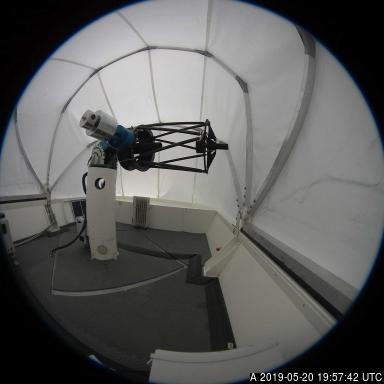
\includegraphics[height=0.6\linewidth]{figures/coatli-webcam-a.jpg}
\fi
\ifddoti
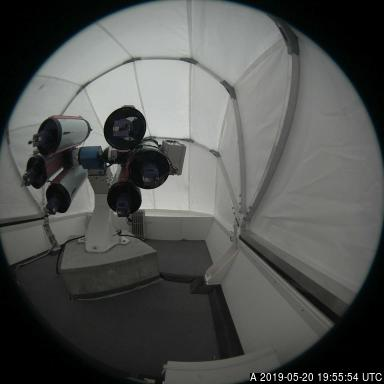
\includegraphics[height=0.6\linewidth]{figures/ddoti-webcam-a.jpg}
\fi
\end{center}
\caption{Typical daytime view from {\projectname} webcam A.}
\label{figure:webcam-a-view}
\begin{center}
\ifcoatli
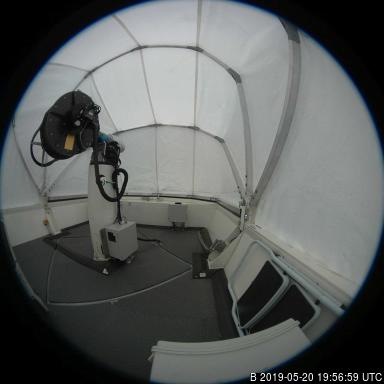
\includegraphics[height=0.6\linewidth]{figures/coatli-webcam-b.jpg}
\fi
\ifddoti
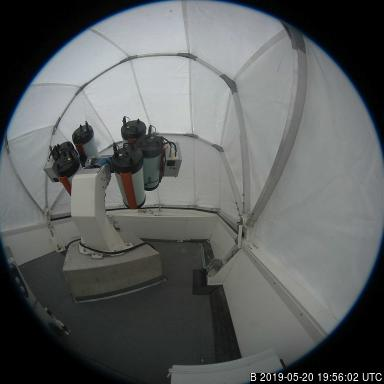
\includegraphics[height=0.6\linewidth]{figures/ddoti-webcam-b.jpg}
\fi
\end{center}
\caption{Typical daytime view from {\projectname} webcam B.}
\label{figure:webcam-b-view}
\end{figure}

\begin{figure}[t]
\begin{center}
\ifcoatli
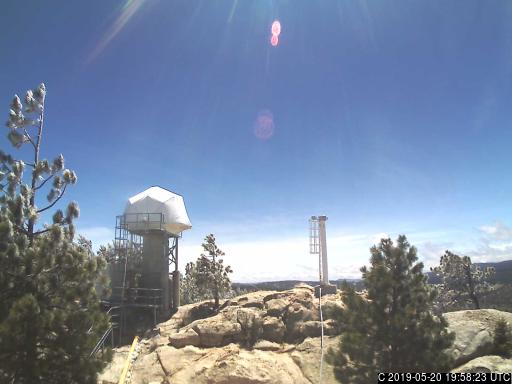
\includegraphics[height=0.6\linewidth]{figures/coatli-webcam-c.jpg}
\fi
\ifddoti
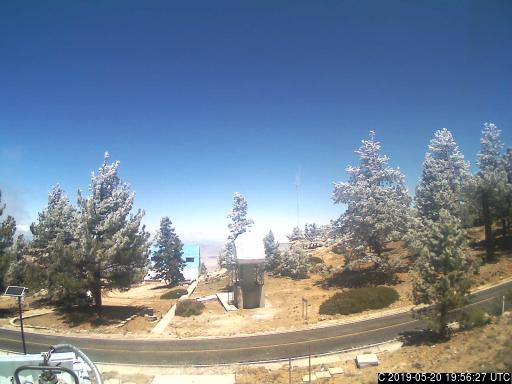
\includegraphics[height=0.6\linewidth]{figures/ddoti-webcam-c.jpg}
\fi
\end{center}
\caption{Typical daytime view from {\projectname} webcam C.}
\label{figure:webcam-c-view}
\begin{center}
\ifcoatli
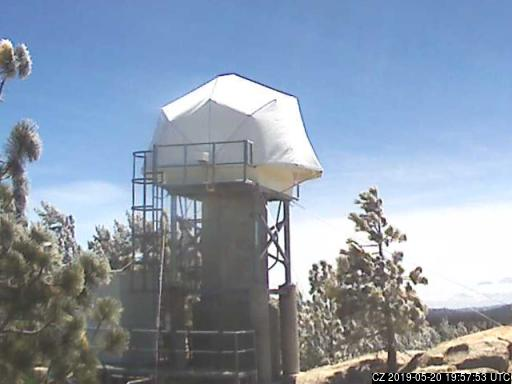
\includegraphics[height=0.6\linewidth]{figures/coatli-webcam-cz.jpg}
\fi
\ifddoti
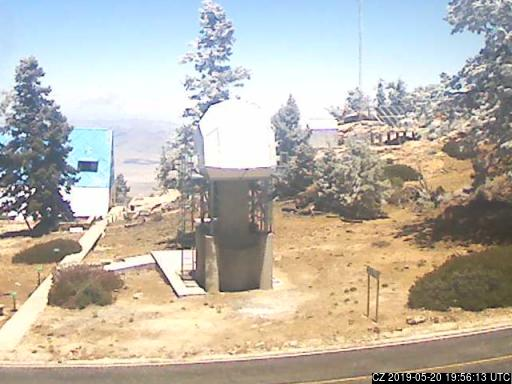
\includegraphics[height=0.6\linewidth]{figures/ddoti-webcam-cz.jpg}
\fi
\end{center}
\caption{Typical daytime view from {\projectname} webcam CZ (en electronic zoom of webcam C).}
\label{figure:webcam-cz-view}
\end{figure}

\section{Platform Webcams}

There are two webcams installed on short posts on the platform. Webcam A is installed above Box B and webcam B is installed above Box C. Figures~\ref{figure:webcam-a-view} and \ref{figure:webcam-b-view} show typical daytime views from webcams A and B. Between them, they can see all of the platform. The platform remote light allow the webcams to monitor the platform even at night. The webcams are Vivotek FE8174V with a 180 degree field of view. This model has an IP66-rated weatherproof housing and can operate down to $-40$~C.

The platform webcams are on the LAN at the addresses given in Table~\ref{table:network-addresses}. The web interfaces can be accessed with the “\projectaccount” account with password “\projectaccount”.

\section{External}

Webcam C is installed on the outside wall of the 84-cm, above the balcony, giving a view of the {\projectname} enclosure. An electronic zoom of webcam C, that shows the enclosure in more detail, is known as webcam CZ. Figures~\ref{figure:webcam-c-view} and \ref{figure:webcam-cz-view} show typical daytime views from webcams C and CZ.
The webcam is a Vivotek MD7560D with a $98 \times 73$ degree field of view lens. This model has an IP67-rated weatherproof housing and can operate down to $-25$~C.

The external webcam in on the observatory public network at the address given in Table~\ref{table:network-addresses}. The web interfaces can be accessed with the “\projectaccount” account with password “\projectaccount”.

\section{Bibliography}

\begin{flushleft}
\begin{itemize}
\item “\href{bibliography/vivotek-fe8174v-data-sheet.pdf}{FE8174/74V Data Sheet}”, Vivotek.
\item “\href{bibliography/vivotek-fe8174v-manual.pdf}{FE8174V User’s Manual}”, Vivotek.
\item “\href{bibliography/vivotek-md7560-alignment-sticker.pdf}{MD7530/60 MD8562/62D Alignment}”, Vivotek.
\item “\href{bibliography/vivotek-md7560-data-sheet.pdf}{MD7560/60D Data Sheet}”, Vivotek.
\item “\href{bibliography/vivotek-md7560-manual.pdf}{MD7530/7530D MD7560/7560D User’s Manual}”, Vivotek.
\item “\href{bibliography/vivotek-md7560-quick-instaltion-guide.pdf}{MD7530/7530D MD7560/7560D Quick Installation Guide}”, Vivotek.
\end{itemize}
\end{flushleft}
